% !TeX root = ../../../../../thesis.tex

\subsubsection{Custom AC Modulator}






Given the shortcomings of the existing hardware, it was decided to build custom hardware that would behave exactly how it was needed in order to successfully encode information in such a way that the currents could be decoded by a smart-meter.
This means that the current signature should behave very similar to the DC case: For a `0' data bit encoding, the current should be zero and for a `1' data bit encoding, the current should be some constant value.
The transitions between the symbols must be such, that a square wave of current will be created, just like in the DC case. 

\begin{figure}[h]
	\centering
	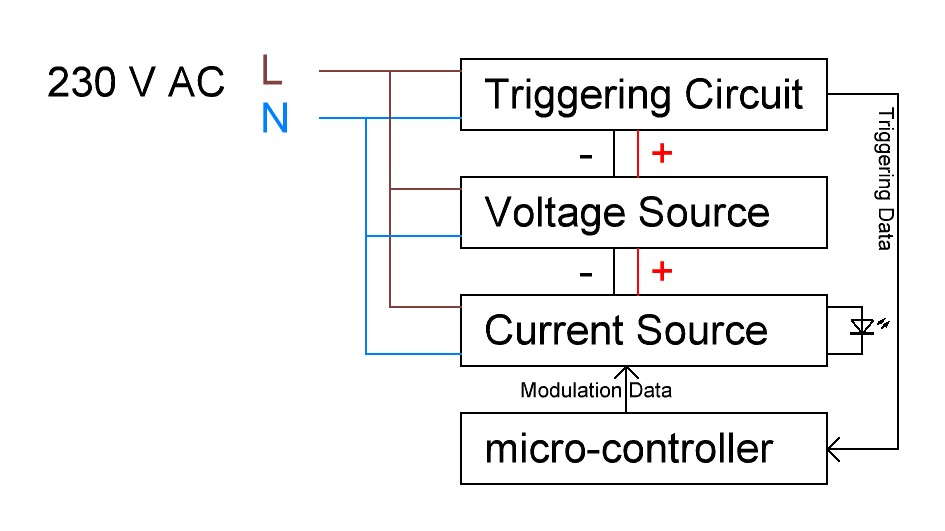
\includegraphics[angle=0,width=0.7\textwidth]{chapters/hardware-chapters/AC/ac-modulator/custom-hardware/ac-modulator-architectural.JPG}
	\caption{Architectural overview of the AC LED modulator.}
	\label{fig:ac-led-modulator-architectural}
\end{figure}

The custom modulator consists of three separate parts: A trigger circuit, a current source and a voltage source.
In \autoref{fig:ac-led-modulator-architectural}, an overview of how these parts are connected to each other can be seen.
The commercial LED that will be used for this solution was already shown \autoref{fig:ac-smps-led-and-smps-picture}, but the SMPS is not used, instead this custom hardware will be powering the LED. 
The entire modulator's schematic can be found in \autoref{app:custom-led-modulator-schematic}.
In the following subsections each part of the hardware of the custom LED modulator will be explained.



	\subparagraph{Triggering}
	\label{subsubsec:triggering}

	As discussed in \autoref{subsubsec:ac-230v-led}, LEDs need a certain amount of voltage before they draw current.
	That is why Figure \ref{fig:commercial-230v-ac-led-on-annotated} has two separate regions where it draws current, instead of drawing current continuously.
	Given the fact that the ID of the LED cannot be transmitted the entire time, due to voltage issue, we must somehow give the micro-controller a signal for when the modulation can start and stop.
	If the micro-controller does not have this information, bits of the ID would be encoded when there is not current draw and thus information would be lost.

	To let the micro-controller know when to start and stop modulating, a triggering circuit is designed.
	This circuit tells the micro-controller when more than a preset voltage is made available by the AC power.
	It also tells the micro-controller when there is less than the preset voltage available.
	In \autoref{fig:triggering-circuit-output-2} the AC voltage can be seen, along with the preset voltage and the corresponding logical output of the triggering circuit.

	%\begin{figure}[h]
	%	\centering
	%	\begin{minipage}[b]{0.39\textwidth}
	%		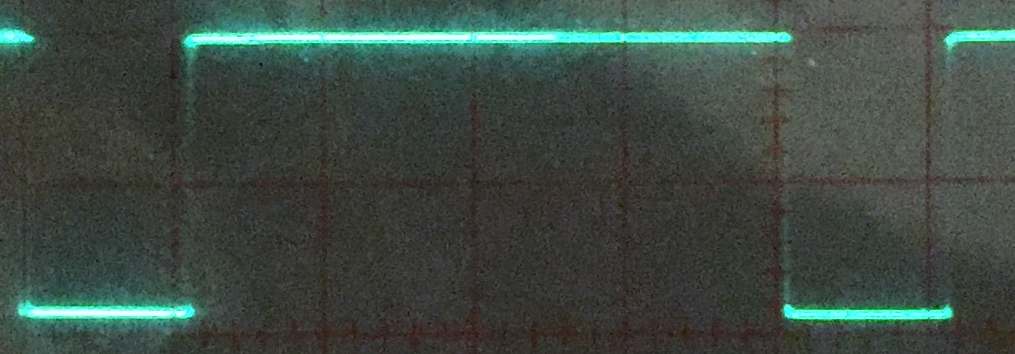
\includegraphics[width=\textwidth]{chapters/hardware-chapters/AC/ac-modulator/custom-hardware/triggering-circuit-output-cropped.png}
	%		\caption{Output from the triggering circuit. Settings: 2 V/div, 2 ms/div.}
	%		\label{fig:triggering-circuit-output}
	%	\end{minipage}
	%	\hfill
	%	\begin{minipage}[b]{0.49\textwidth}
	%		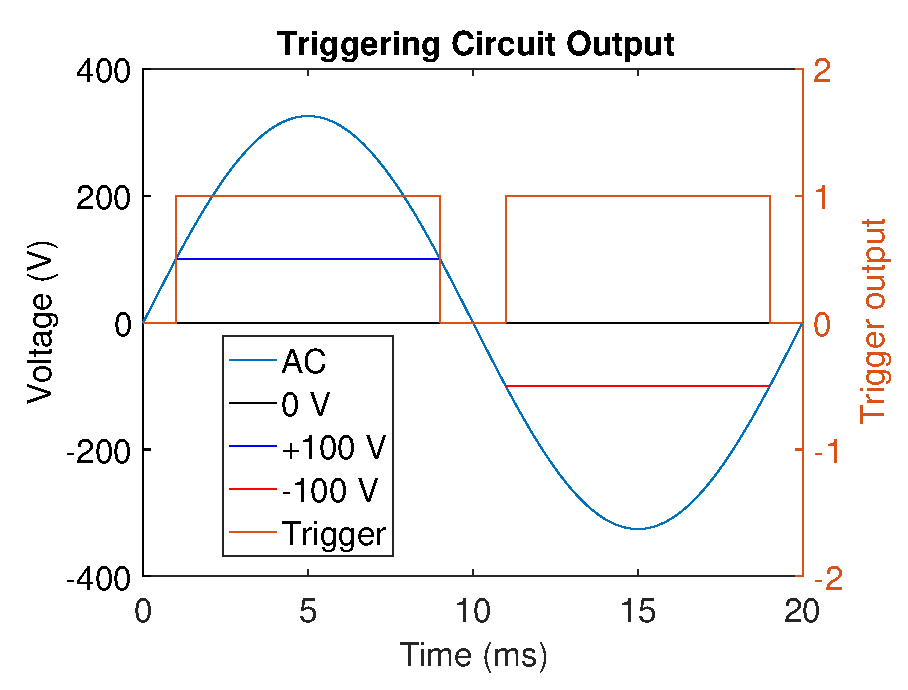
\includegraphics[width=\textwidth]{chapters/hardware-chapters/AC/ac-modulator/custom-hardware/ac-wave-triggering.eps}
	%		\caption{Output form the triggering circuit alongside the incoming AC voltage.}
	%		\label{fig:triggering-circuit-output-2}
	%	\end{minipage}
	%\end{figure}


	\begin{figure}[h]
		\centering
		\begin{minipage}[b]{0.49\textwidth}
			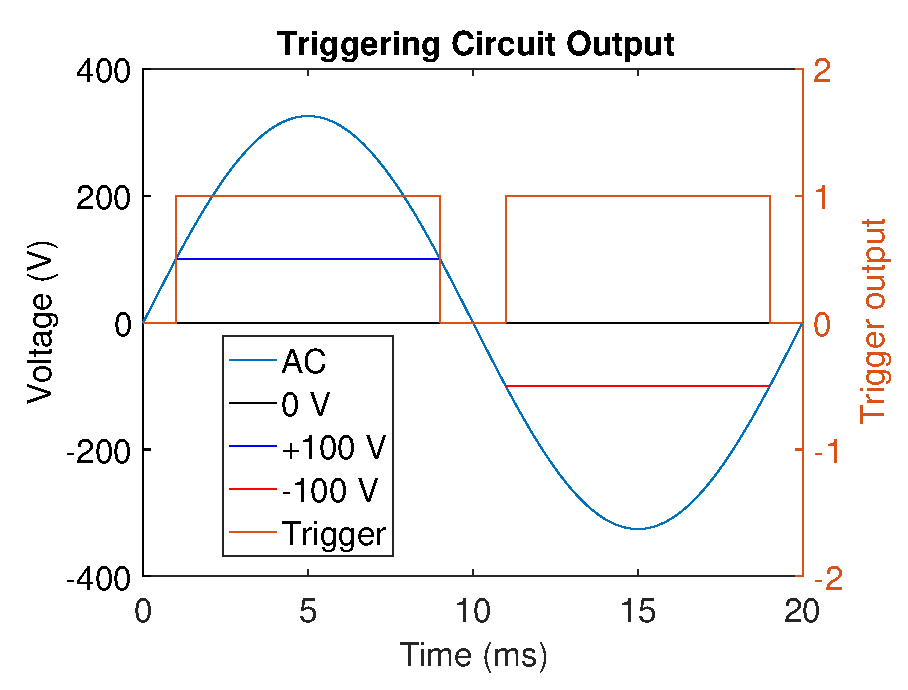
\includegraphics[width=\textwidth]{chapters/hardware-chapters/AC/ac-modulator/custom-hardware/ac-wave-triggering.eps}
			\caption{Output form the triggering circuit alongside the incoming AC voltage.}
			\label{fig:triggering-circuit-output-2}
		\end{minipage}
		\hfill
		\begin{minipage}[b]{0.49\textwidth}
			\includegraphics[width=\textwidth]{chapters/hardware-chapters/AC/ac-modulator/custom-hardware/custom-modulator-trigger.JPG}
		    \caption{Triggering circuit to determine when the voltage is sufficiently high enough to start encoding the ID.}
			\label{fig:custom-modulator-trigger}
		\end{minipage}
	\end{figure}

	In \autoref{fig:triggering-circuit-output-2}, the preset voltage is set at 100 V.
	When more than 100 V is available the LED will emit light and start drawing current.
	At that point, around 1 ms in the figure, the triggering circuit will output a logical `1' to the micro-controller, meaning that the encoding of the ID may start.
	When less than 100 V is available, around 9 ms in the figure, the logical output of the circuit becomes `0', indicating to the micro-controller that it is time to stop encoding the ID, because else information is lost since the LED is not turning on anymore.
	The same happens for the negative part of the sine wave, except the preset is now $-100$ V.


	From \autoref{fig:triggering-circuit-output-2} it can be deduced that two times 8 ms is available to encode the ID in a period of 20 ms.
	So $\frac{2 \times 8}{20} = 80$ \% of the time is available for modulation, which is two times more than the solution in \autoref{subsubsec:ac-230v-led} provided.
	To transmit the ID, this solution would be two times faster, but it would still take 25 \% more time than in a DC environment.



	In \autoref{fig:custom-modulator-trigger}, the circuit can be seen which signals the micro-controller when the voltage is more or less than the preset voltage. 
	The voltage preset can be set by using a potentiometer.
	The output of the circuit is electrically isolated from the micro-controller by the means of an optocoupler.
	This is done to protect the micro-controller from the high voltage AC in the development stages.








	


	




	%Both figure side by side to save space...
	%\begin{figure}[!tbp]
	%  \centering
	%  \begin{minipage}[b]{0.48\textwidth}
	%    \includegraphics[width=\textwidth]{chapters/hardware-chapters/custom-modulator-trigger.JPG}
	%    \caption{Triggering circuit to determine when the voltage is sufficiently high enough to start encoding information.}
	%	\label{fig:custom-modulator-trigger}
	%  \end{minipage}
	%  \hfill
	%  \begin{minipage}[b]{0.48\textwidth}
	%    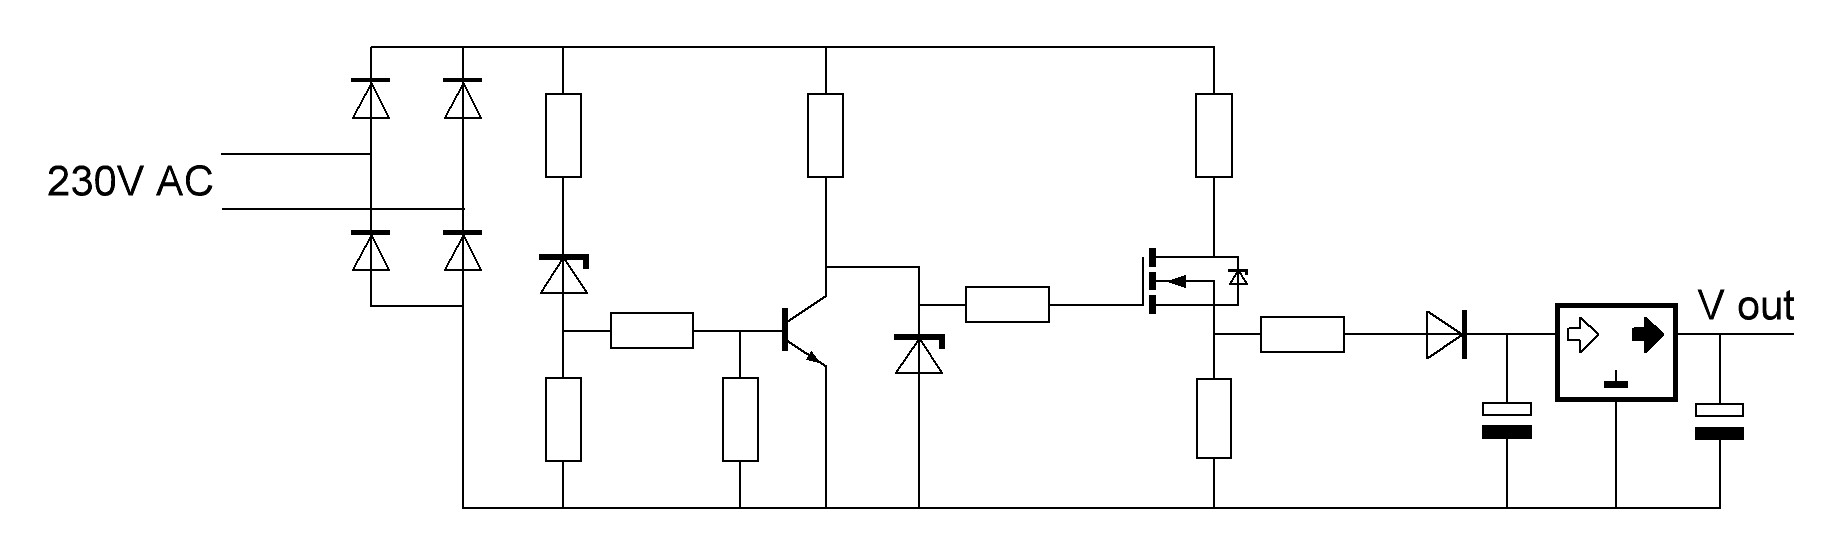
\includegraphics[width=\textwidth]{chapters/hardware-chapters/custom-modulator-voltage-source.JPG}
	%    \caption{Non-disturbing voltage source to power other parts of the circuit.}
	%	\label{fig:custom-modulator-voltage-source}
	%  \end{minipage}
	%\end{figure}

	\subsubsection{Non-disturbing Voltage Source}
	\label{subsubsec:non-disturbing-voltage-source}

	The triggering circuit (\autoref{fig:custom-modulator-trigger}) requires a 5 V power supply.
	This voltage must be provided by a voltage source that will not distort the current draw.
	Otherwise it might disturb how the code sequence is translated in the current draw.

	Since the triggering circuit determines when the encoding may start, the voltage source can operate before the encoding starts.
	In that way it will not distort the encoding, because no encoding takes place yet.
	The schematic found in \autoref{fig:custom-modulator-voltage-source} provides a stable 5 V output.
	By only drawing current when there is no encoding being done, the voltage that the AC is providing is low, but still above 5 V.
	The AC voltage is then being used to charge a capacitor, that goes to a voltage stabilizer.
	The capacitor can then provide enough power for the triggering circuit until the capacitor can be charged again.


	%\begin{figure}[htb]
	%	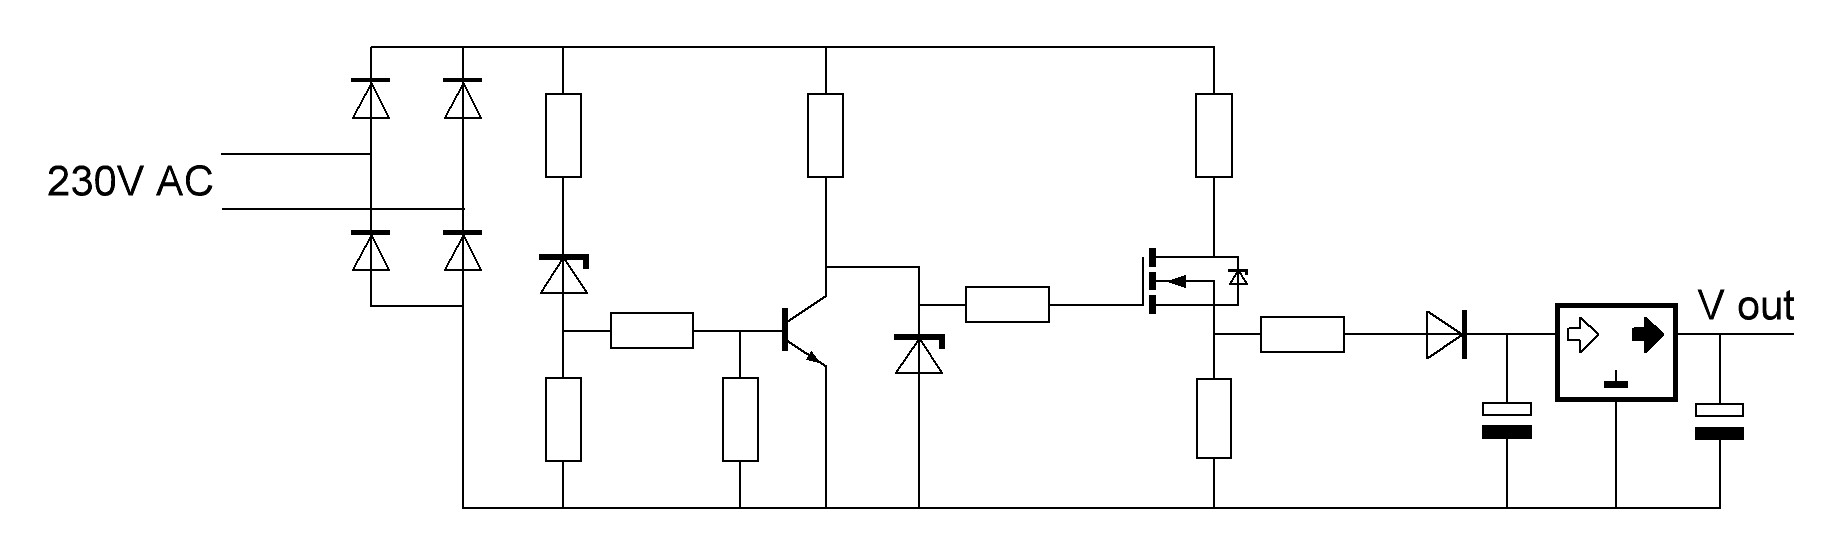
\includegraphics[angle=0,width=\textwidth]{chapters/hardware-chapters/custom-modulator-voltage-source.JPG}
	%	\caption{Non-disturbing voltage source to power other parts of the circuit.}
	%	\label{fig:custom-modulator-voltage-source}
	%\end{figure}



	\subsubsection{Current Source}
	\label{subsubsec:current-source}


	For the current to be drawn instantaneously when the microprocessor tells the LED to turn on and to always be the same amount of current, a current source is implemented. 
	This will solve the problems that the other solutions have, such as: a non-constant current draw and a non-instantaneous current draw but a slope.
	The toggling of the current source on and off must be isolated from the microprocessor, to protect the microprocessor in the development stages, for this an optocoupler is used.
	The schematic can be found in \autoref{fig:custom-modulator-current-source}.
	The current that is drawn by the current source when modulating can be seen in \autoref{fig:current-source-measurement}.
	As seen in the figure the current goes both positive and negative, because of the AC, but the current itself is always a constant value, no matter if the current source is on or off.
	The two peaks in the figure are the charging peaks for the capacitors as discussed in \autoref{subsubsec:non-disturbing-voltage-source}.


	However, this solution also has a drawback.
	The current source will make sure a constant amount of current will flow through the LEDs.
	The current that flows through the LEDs will cause a voltage difference over the LEDs.
	This is the voltage the LEDs need in order to be turned on, as discussed in \autoref{subsubsec:triggering}.
	The rest of the voltage that the AC delivers will have to go somewhere.
	This voltage will be dissipated over the current source.
	This means that some energy is now being wasted, because there is more voltage provided by the AC than is needed to power the LEDs.

	One solution for this is using a transformer.
	This will scale down the voltage, but it will still remain a sinusoidal wave.
	But the same amount of voltage is still required by the LEDs.
	And if the sine wave now has a smaller amplitude, the time that is left for modulation will also be much smaller.
	This can be seen in \autoref{fig:trigger-output-lower-transformed}.
	Here the same voltage is required by the LEDs, 100 V.
	But the incoming sine wave has a smaller amplitude because a transformer, transformed the 230 V AC to a lower voltage.
	The time that is now available for modulation is 6 ms, which means that only $\frac{6}{20} = 30$ \% of the time is now available for modulation.
	Another drawback is that the transformer will deform the distinct current pattern that we are trying to create, as no ideal transformers exist.

	Another solution was thought of and also implemented in the circuit boards but due to lack of time it was not further experimented with.
	The solution is made up out of two parts: A capacitor and a zero-crossing opto-triac.
	The capacitor is place in series with incoming AC to the rectifying bridge.
	And the opto-triac is parallel to this capacitor.
	The schematic can be seen in \autoref{fig:ac-capacitor-triac}.
	The capacitor with AC acts as a kind of resistor so it will limit the power that is dissipated by the current source, but the capacitor itself will not dissipate any power.
	However by limiting the power that the current source will dissipate the amplitude of the sine will also become smaller and then there is much less time available to modulate, similar to the solution with the transformer as described above.
	This is were the zero-crossing triac comes in.
	Whenever it is decided to start modulating, the microcontroller activates the triac and then it will short-circuit the capacitor when the voltage is zero, so that no current will flow through the triac and thereby not damaging the triac.
	Now the capacitor is bypassed and modulation can begin with a large time available for modulation.
	When the modulation is done, the triac is switched off and the capacitor limits the power once again.
	The drawback that comes with this is that the capacitor can limit the power by phase-shifting the current as seen from the voltage.
	But the current will not be phase-shifted when the triac is active.
	So this solution is a complicated one, but it can solve the problem that the current source is dissipating excessive power.
	But it also introduces a lot of complexity and there was no more time to evaluate the benefits and drawbacks of this solution.




	%\begin{figure}
	%	\centering
	%	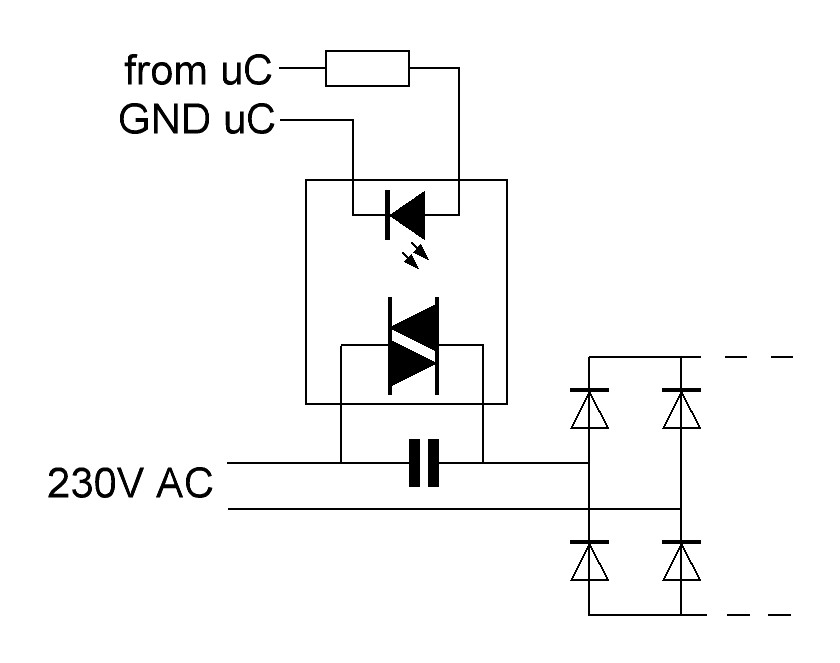
\includegraphics[angle=0,width=0.5\textwidth]{chapters/hardware-chapters/ac-capacitor-triac.JPG}
	%	\caption{Schematic to show how the capacitor and opto-triac are connected.}
	%	\label{fig:ac-capacitor-triac}
	%\end{figure}


	%\begin{figure}[!tbp]
	%  \centering
	%  \begin{minipage}[b]{0.49\textwidth}
	%    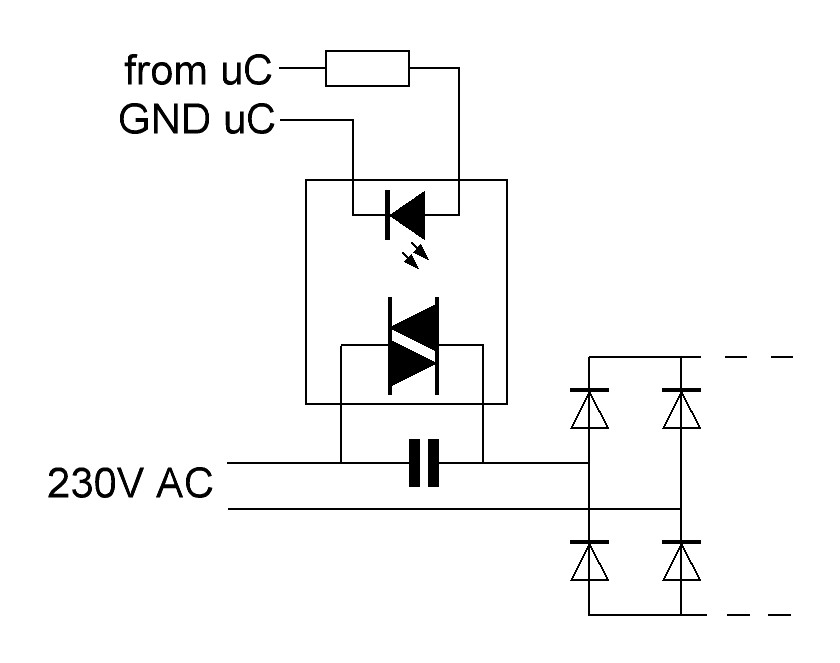
\includegraphics[width=\textwidth]{chapters/hardware-chapters/ac-capacitor-triac.JPG}
	%	\caption{Schematic to show how the capacitor and opto-triac are connected.}
	%	\label{fig:ac-capacitor-triac}
	%  \end{minipage}
	%  \hfill
	%  \begin{minipage}[b]{0.49\textwidth}
	%    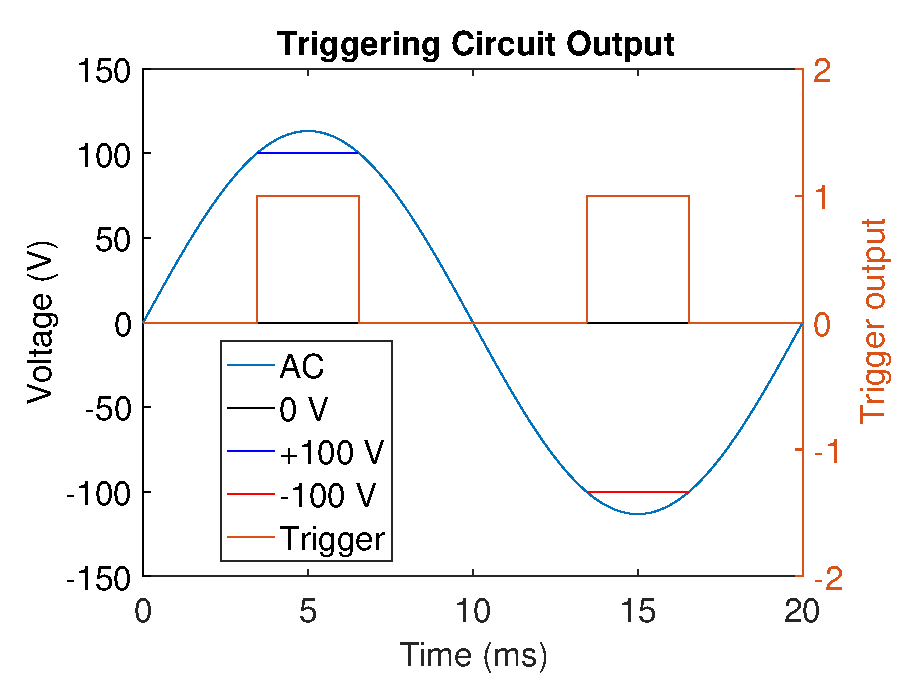
\includegraphics[width=\textwidth]{chapters/hardware-chapters/ac-wave-lower-transformed-triggering.eps}
	%    \caption{Output triggering circuit alongside the output of the AC voltage after a transformer.}
	%    \label{fig:trigger-output-lower-transformed}
	%  \end{minipage}
	%\end{figure}
%
%
%	%%\begin{figure}[htb]
%	%%	\centering
%	%%	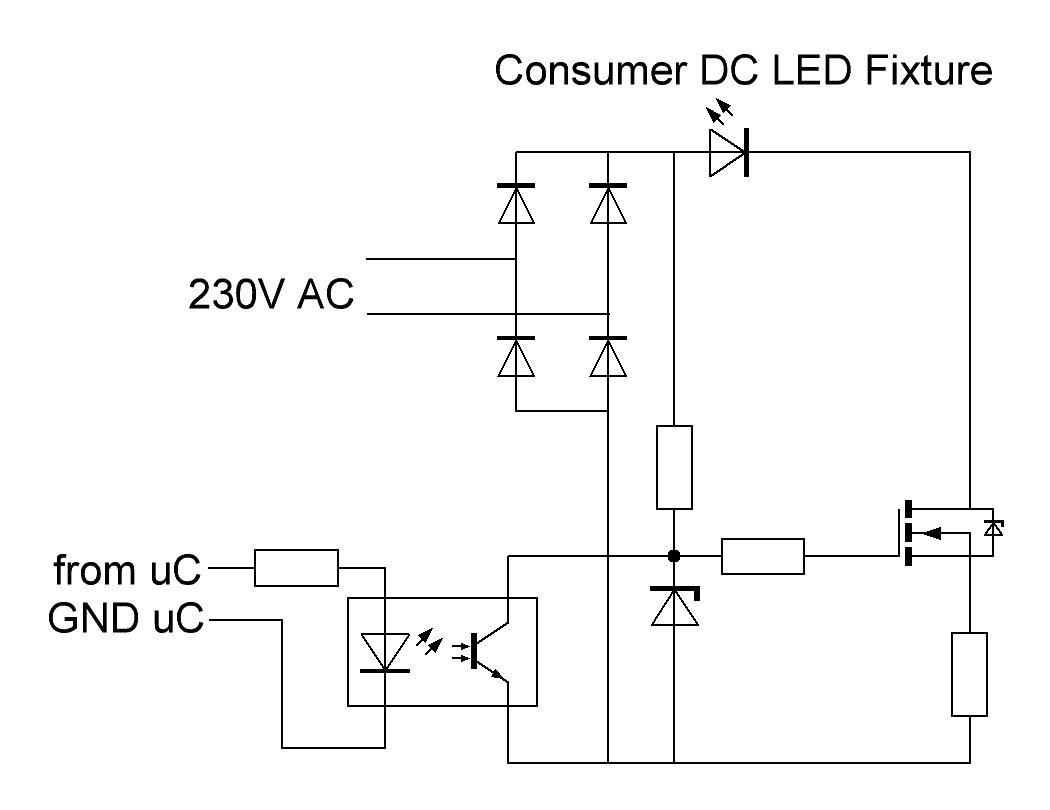
\includegraphics[angle=0,width=0.5\textwidth,keepaspectratio]{chapters/hardware-chapters/custom-modulator-current-source.JPG}
%	%%	\caption{Current source to power the commercial LED fixture, can be toggled on and off with a microprocessor.}
%	%%	\label{fig:custom-modulator-current-source}
%	%%\end{figure}
%
%	%\begin{figure}[!tbp]
%	%  \centering
%	%  \begin{minipage}[b]{0.49\textwidth}
%	%    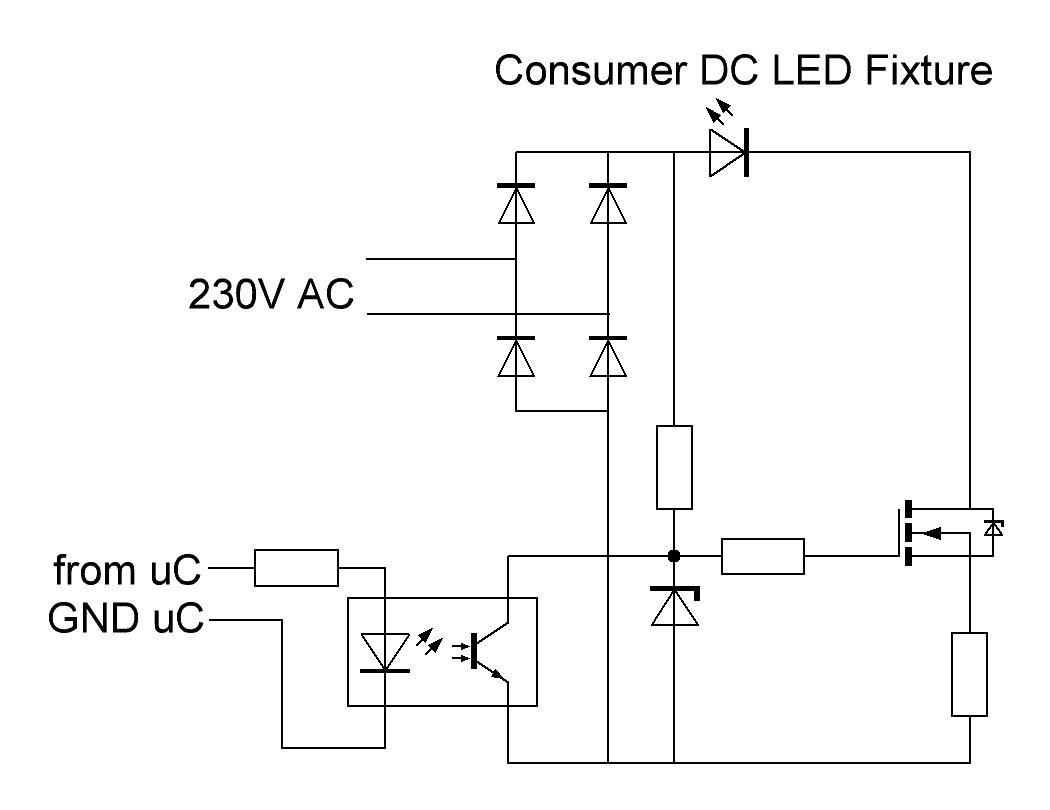
\includegraphics[width=\textwidth]{chapters/hardware-chapters/custom-modulator-current-source.JPG}
%	%	\caption{Current source to power the commercial LED fixture, can be toggled on and off with a microprocessor.}
%	%	\label{fig:custom-modulator-current-source}
%	%  \end{minipage}
%	%  \hfill
%	%  \begin{minipage}[b]{0.49\textwidth}
%	%    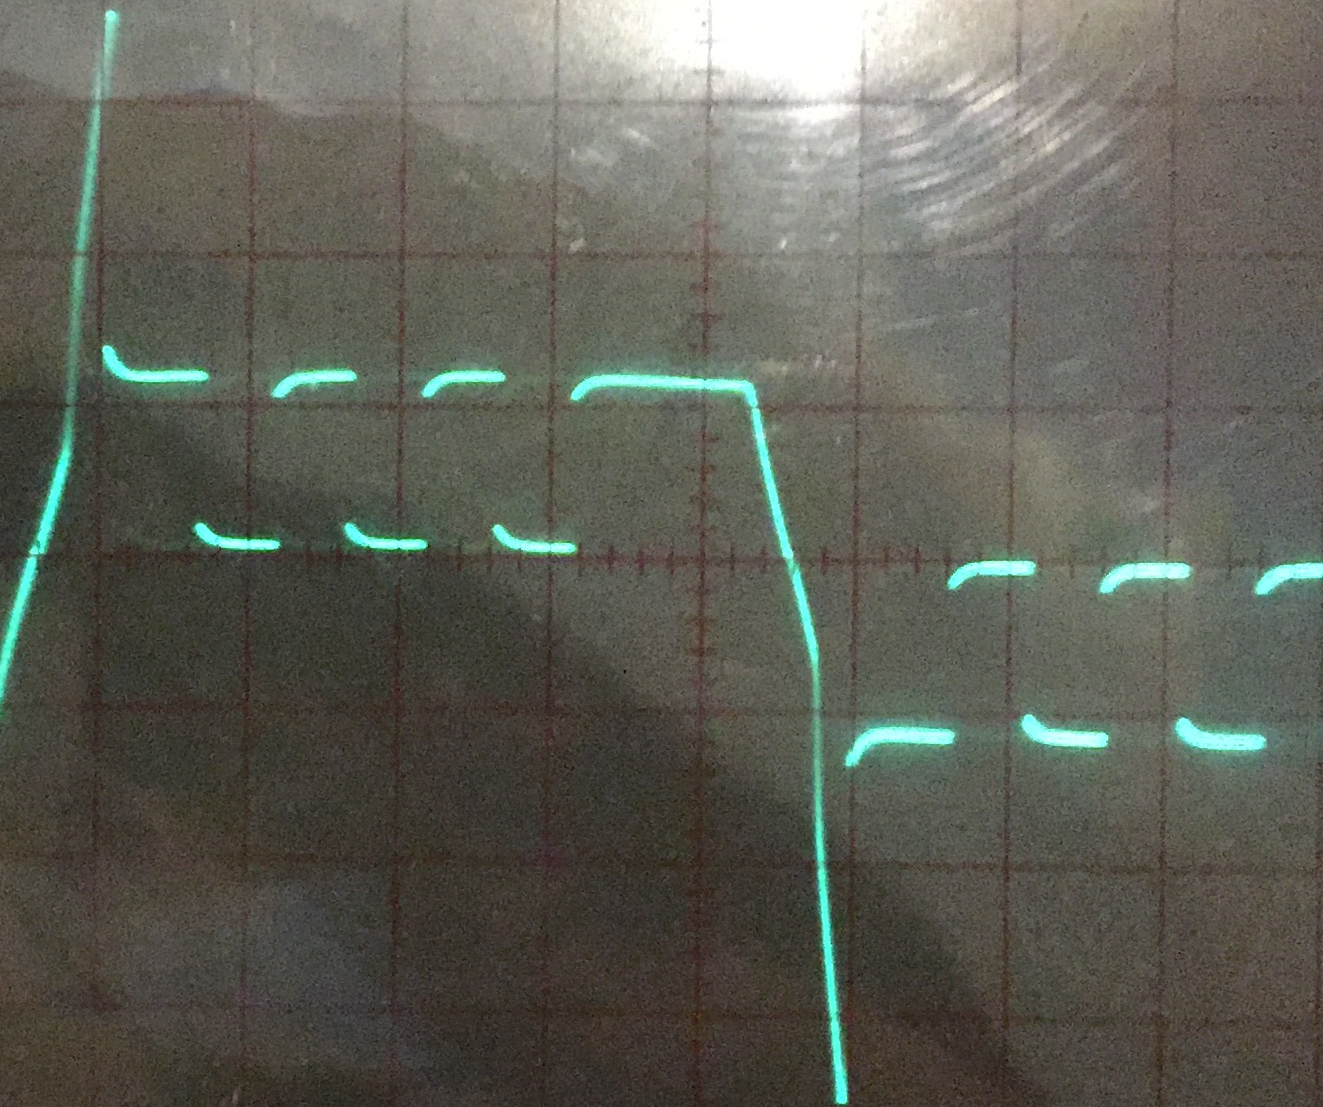
\includegraphics[width=\textwidth]{chapters/hardware-chapters/current-source-measurement-cropped.png}
%	%    \caption{Current that is drawn by the current source. Measured over an 2.8 Ohm resistor. Settings: 200 mV/div, 2 ms/div.}
%	%	\label{fig:current-source-measurement}
%	%  \end{minipage}
%	%\end{figure}
%